相互作用网络是很有用的模型,但是,如果能跟其它信息整合在一起,则能解答更多的科学疑问。在Cytoscape中,用户可以给节点、边或网络添加各种属性。例如,可以是基因的注释数据或蛋白质相互作用的可信度。这些属性可以按着用户的设置映射到可视化属性上(颜色、形状等等)。本节会详细介绍视觉风格。

\section{Cytoscape~属性文件格式}
节点和边的属性文件的格式非常简单:节点属性文件的第一行是属性的名称(注意,属性名称中不能有空格)。接下来的每一行首先是节点的名称,然后是等号,以及属性的值。最常见的属性类型是数字和字符串。同一个属性的所有值都必须是同一类型的。例如:

 \begin{verbatim}
FunctionalCategory
YAL001C = metabolism
YAR002W = apoptosis
YBL007C = ribosome
\end{verbatim}

边的属性文件也类似,不同的是边的名称是由起点名称,加上括号中的边的类型,然后是重点名称构成的。边是有方向性的,所以交换起点和终点的位置会被认为是不同的边(有可能是不存在的)。下面就是一个边属性文件的例子:

 \begin{verbatim}
InteractionStrength
YAL001C (pp) YBR043W = 0.82
YMR022W (pd) YDL112C = 0.441
YDL112C (pd) YMR022W = 0.9013
\end{verbatim}

在Cytoscape中,边是有方向的,所以上表中的第三行和第四行表示的是两条不同的边(涉及到的节点是一样的,但终点和起点是相反的)。

每个文件存放一个属性。节点和边的属性文件的格式是一样的。节点属性文件名的后缀一般是
``.noa'',边属性文件名的后缀通常是``.eda''。这两个后缀都能被Cytoscape识别。

可以用命令行的-n和-e选项或菜单中的File $\rightarrow$ Import加载节点和边的属性。

如果通过基因表达矩阵加载了基因表达数据,在缺省情况下,其表达值会自动地转换成节点的属性。

节点和边的属性只跟节点和边有关,是独立于网络的。无论是先加载网络文件还是先加载属性文件,节点或边的属性都会应用到当前加载的所有网络中。

\textbf{注意:}在Cytoscape 2.4中导入网络属性时,请使用File $\rightarrow$ Import $\rightarrow$ Attribute from Table (text/MS Excel)...或XGMML格式的网络文件(相见所支持的文件格式一章)。

\subsection{符号分割文件格式(高级用户)}

该格式的属性文件的第一行说明了属性的名称以及该属性的附加信息,如下:

\begin{verbatim}
attributeName (class=formal.class.of.value)
\end{verbatim}

第一个字段必须是属性名称,并且不能含有空格。class字段定义了属性值的正式类型。例如,
java.lang.String表示字符串、java.lang.Double表示浮点数值、java.lang.Integer表示整数,以此类推。
如果值是一份列表,那么class字段就应该是列表中对象的类型。如果没有指定class字段,Cytoscape
就会根据文件中的第一个值猜测其类型。如果第一个值中含有浮点格式的数字,Cytoscpae就会认为是
java.lang.Double;如果第一个值只有数字,没有小数点,Cytoscape就会认为是java.lang.Integer;除此以外,Cytoscape
都会将其视为java.lang.String。所以,要小心,第一个值可能会造成Cytoscape的错误,例如:

 \begin{verbatim}
floatingPointAttribute
firstName = 1
secondName = 2.5
\end{verbatim}

在上面的例子中,第一个值会导致Cytoscape将该属性的类型设为整数,但实际上其类型应该是
浮点数。所以最好是明确地指定属性的类型,以避免这种错误。如下:

 \begin{verbatim}
floatingPointAttribute (class=Double)
firstName = 1
secondName = 2.5
\end{verbatim}

或者:

 \begin{verbatim}
floatingPointAttribute 
firstName = 1.0
secondName = 2.5
\end{verbatim}

Every line past the first line identifies the name of an object (a node in a
node attribute file or an edge in a edge attribute file) along with the String
representation of the attribute value. The delimiter is always an equals sign;
whitespace (spaces and/or tabs) before and after the equals sign is ignored.
This means that your names and values can contain whitespace, but object names
cannot contain an equals sign and no guarantees are made concerning leading or
trailing whitespace. Object names must be the Node ID or Edge ID as seen in the
left-most column of the attribute browser if the attribute is to map to
anything. These names must be reproduced exactly, including case, or they will
not match. 

Edge names are all of the form: 

 \begin{verbatim}
sourceName (edgeType) targetName
\end{verbatim}

 Specifically, that is 

 \textbf{Table\^A 10.\^A }

\begin{tabular}{|c|}
 \hline 
 sourceName space openParen edgeType closeParen space targetName \\
 \hline 
\end{tabular}

 Note that tabs are not allowed in edge names. Tabs can be used to separate the
edge name from the ``='' delimiter, but not within the edge name itself. Also
note that this format is different from the specification of interactions in
the SIF file format. To be explicit: a SIF entry for the previous interaction
would look like 

 \begin{verbatim}
sourceName edgeType targetName
\end{verbatim}

 or 

 \textbf{Table\^A 11.\^A }
\begin{tabular}{|c|}
\hline 
 sourceName whiteSpace edgeType whiteSpace targetName \\
\hline 
\end{tabular}

 To specify lists of values, use the following syntax: 

 \begin{verbatim}
listAttributeName (class=java.lang.String)
firstObjectName = (firstValue::secondValue::thirdValue)
secondObjectName = (onlyOneValue)
\end{verbatim}

 This example shows an attribute whose value is defined as a list of text
strings. The first object has three strings, and thus three elements in its
list, while the second object has a list with only one element. In the case of
a list every attribute value uses list syntax (i.e. parentheses), and each
element is of the same class. Again, the class will be inferred if it is not
specified in the header line. Lists are not supported by the visual mapper and
so can't be mapped to visual attributes. 

\subsection{Newline Feature}
Sometimes it is desirable to for attributes to include linebreaks, such as node
labels that extend over two lines. You can acomplish by inserting   into the
attribute value. For example: 

 \begin{verbatim}
newlineAttr
YJL157C = This is a long\nline for a label.
\end{verbatim}

\subsection{导入属性表格文件}

 As of Cytoscape 2.4, importing delimited text and MS Excel attribute data
tables is now supported. Using this functionality, users can now easily import
data that isn't formatted into Cytoscape node or edge attribute file formats
(as described above). 

\centerline{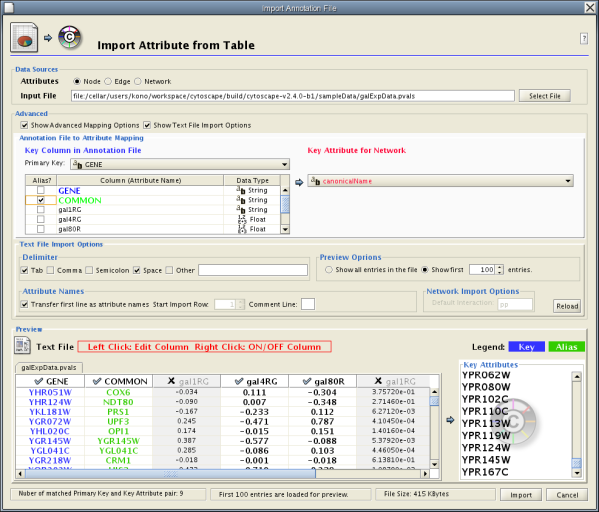
\includegraphics[width=.6\textwidth]{images/attribute_table_import_main.png} }

 \emph{\textbf{Sample Attribute Table 1} }

 \textbf{Table 12. }

\begin{tabular}{|c|c|c|}
\hline 
 Object& Key Alias& SGD ID\\
\hline
 AAC3 &YBR085W|ANC3& S000000289\\
 AAT2 &YLR027C|ASP5& S000004017\\
 BIK1 & YCL029C|ARM5|PAC14 &S000000534\\
 \hline 
\end{tabular}

 The attribute table file should contain a primary key column and at least one
attribute column. The maximum number of attribute columns is unlimited. The
\emph{Alias} column is an optional feature, as is using the first row of data
as attribute names. Alternatively, you can specify each attribute name from the
File$\rightarrow$Import$\rightarrow$Attribute from Table (text/MS Excel)...
user interface. 


 \textbf{Basic Operation}

 The user interface of the ``Import Attributes from Table'' window is similar to that of the ``Import Network from Table'' window. 
\begin{enumerate}
\item Select File $\rightarrow$Import $\rightarrow$Attribute from Table (text/MS
Excel)... 
\item Select one of the attribute types from the Attributes radio buttons.
Cytoscape can import node, edge, and network attributes. 
\item Select a data file. To load a local file, click on the Select File button
and choose a data file. This can be either a text or Excel (.xls) file. To load
a remote file, type the source URL directly into the text box. To show a
preview of the remote file, click the Reload button on the Show Text File
Import Options panel. 
\item (Optional) If the table is not properly delimited in the preview panel,
change the delimiter in the Text File Import Options panel. The default
delimiter is the tab. This step is not necessary for Excel Workbooks. 
\item By default, the first column is designated as the primary key. Change the
key column if necessary.
\begin{itemize}
\item 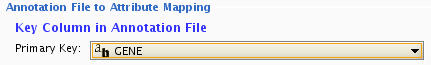
\includegraphics[width=\textwidth]{images/attribute_table_import_primary_key.png} 
\end{itemize}
\item Click the Import button. 
\end{enumerate}
 
\textbf{Advanced Options}
\textbf{Mapping Key Attributes to the primary key}
 Formerly, Cytoscape only supported mapping between node/edge IDs and the
primary keys in attribute files. With the introduction of Cytoscape 2.4, this
limitation has been removed, and now both IDs and attributes with primitive
data types (string, boolean, floating point, and integer) can be selected as
the Key Attribute using the dropdown list provided. Complex attributes such as
lists are not supported. 


 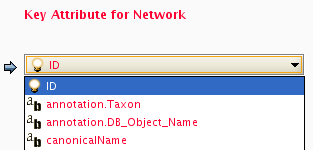
\includegraphics[width=\textwidth]{images/attribute_table_import_keyattr.png} 
 
\subsection{Aliases}

 Cytoscape uses a simple mechanism to manage aliases of objects. Both nodes and
edges can have aliases. If an attribute is loaded as an alias, it is treated as
a special attribute called ``alias''. This will be used when mapping
attributes. If the primary key and key attribute for an object do not match,
Cytoscape will search for a match between aliases and the key attribute. To
define an alias column in the attribute table, just click on the checkboxes to
the left of the column name while importing. 


 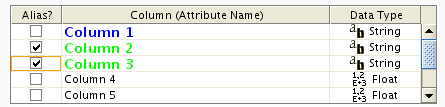
\includegraphics[width=\textwidth]{images/attribute_table_import_alias.png} 


 
\textbf{Text File Import Options}


 For more detail on these options, please see the ``Import Free-Format Table
Files'' section of the user manual in the Creating Networks chapter. 


 

\textbf{Attribute Browser}


 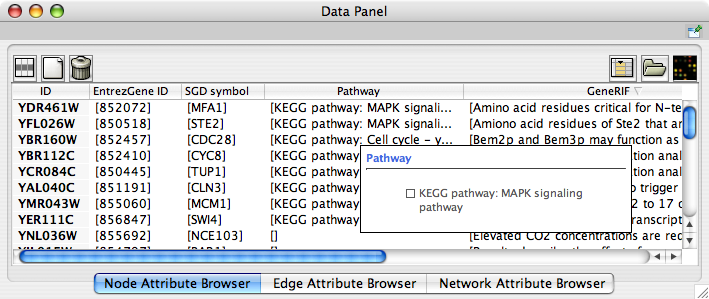
\includegraphics[width=\textwidth]{images/attribute_browser26.png} 


 When Cytoscape is started, the Attribute Browser appears in the bottom
CytoPanel. This browser can be hidden and restored using the F5 key or the View
$\rightarrow$ Show/Hide attribute browser menu option. Like other CytoPanels, the
browser can be undocked by pressing the little icon in the browser's
top right corner. 


 To swap between displaying node, edge, and network attributes use the tabs on
the bottom of the panel labelled ``Node Attribute Browser'', ``Edge Attribute
Browser'', and ``Network Attribute Browser''. The attribute browser displays
attributes belonging to selected nodes and/or edges and the currently selected
network. To populate the browser with rows (as pictured above), simply select
nodes and/or edges in a loaded network. By default, only the ID of nodes and
edges is shown. To display more than just the ID, click the Select Attributes

\includegraphics[scale=1]{images/attributes_select_icon.png}  button and choose
the attributes that are to be displayed (select various attributes by clicking
on them, and then click elsewhere on the screen to close the attribute list).
Each attribute chosen will result in one column in the attribute browser. Most
attribute values can be edited by double-clicking an attribute cell; list
values cannot be edited, and neither can the ID. Attribute rows in the browser
can be sorted alphabetically by specific attribute by clicking on a column
heading. A new attribute can be created using the Create New Attribute

\includegraphics[scale=1]{images/attributes_new_icon.png}  button, and must be
one of four types \^a€“ integer, string, real number (floating point), or
boolean. Attributes can be deleted using the Delete Attributes

\includegraphics[scale=1]{images/attributes_delete_icon.png}  button.
\textbf{NOTE: Deleting attributes removes them from Cytoscape, not just the
attribute browser!} To remove attributes from the browser without deleting
them, simply unselect the attribute using the Select Attributes

\includegraphics[scale=1]{images/attributes_select_icon.png}  button. 


 The right-click menu on the Attribute Browser has several functions, such as
exporting attribute information to spreadsheet applications. For example, use
the right-click menu to Select All and then Copy the data, and then paste it
into a spreadsheet application. Each attribute browser panel also has a button
for importing new attributes:

\includegraphics[scale=1]{images/attributes_import_icon.png}  . 


 The Node Attribute Browser panel has additional buttons for loading Gene
Expression attribute matrices (
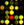
\includegraphics[width=1em]{images/attributes_gene_expr_icon.png}  ) as node
attributes. 


 \textbf{Attribute Batch Editor}


 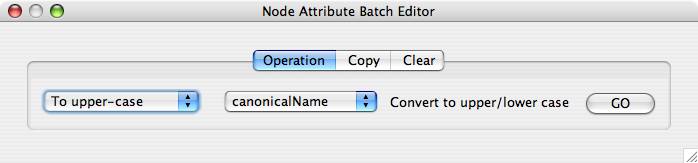
\includegraphics[width=\textwidth]{images/attribute_editor26.png} 


 From Cytoscape 2.6, Attribute Browser has new \textbf{Attribute Batch Editor}
. This enables you to set and modify attribute values at once. This function
changes values for selected nodes or edges. For example, if you want to create
a new attribute called \emph{Modules} and set module names for each group of
selected nodes, you can use \emph{Set} command from this editor. 
